% Канонический TikZ-рисунок варианта 03 и его аналогов.
\newcommand{\figCyclicTrapezoid}{%
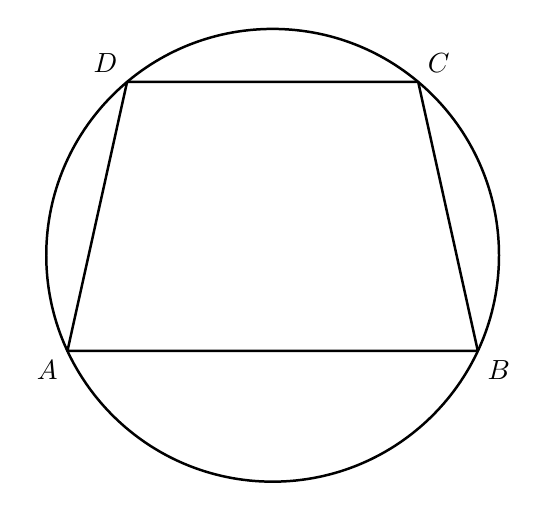
\begin{tikzpicture}[scale=1.15,line cap=round,line join=round]
  \def\R{2.5}
  \coordinate (A) at (205:\R); \coordinate (B) at (335:\R);
  \coordinate (C) at (50:\R); \coordinate (D) at (130:\R);
  \draw[line width=0.9pt] (0,0) circle (\R);
  \draw[line width=0.9pt] (A)--(B)--(C)--(D)--cycle;
  \node[below left] at (A) {$A$}; \node[below right] at (B) {$B$};
  \node[above right] at (C) {$C$}; \node[above left] at (D) {$D$};
\end{tikzpicture}}
